\documentclass{article}

\usepackage{corl_2023} % Use this for the initial submission.
%\usepackage[final]{corl_2023} % Uncomment for the camera-ready ``final'' version.
%\usepackage[preprint]{corl_2023} % Uncomment for pre-prints (e.g., arxiv); This is like ``final'', but will remove the CORL footnote.

% ### custom packages start ###
% math
\usepackage{amsmath,amsfonts,amssymb,amsthm}
\usepackage{mathtools}
\usepackage{commath}
\DeclareMathOperator*{\argmax}{arg\,max}
\DeclareMathOperator*{\argmin}{arg\,min}

% tables
\usepackage{array}
\usepackage{booktabs}
\usepackage{multirow}

% figures
\usepackage{subcaption}
\usepackage{wrapfig}

% algorithms
\usepackage{algorithm}
\usepackage{algpseudocode}
\newcommand{\minuseq}{\mathrel{-}=}

% colors
\usepackage{xcolor}
\newcommand{\ob}[1]{\textcolor{purple}{[\textbf{OB:} #1]}}
\newcommand{\evdp}[1]{\textcolor{blue}{[\textbf{EvdP:} #1]}}
\newcommand{\lsw}[1]{\textcolor{olive}{[\textbf{lsw:} #1]}}

% highlight
\usepackage{soul}
\definecolor{lightlightgrey}{rgb}{0.9,0.9,0.9}
\sethlcolor{lightlightgrey}
% ### custom packages end ###

\title{SA-Warp: Simple $\mathrm{SE}(3)$ Object Re-arrangement \\via Shape and Action Warping}

% The \author macro works with any number of authors. There are two
% commands used to separate the names and addresses of multiple
% authors: \And and \AND.
%
% Using \And between authors leaves it to LaTeX to determine where to
% break the lines. Using \AND forces a line break at that point. So,
% if LaTeX puts 3 of 4 authors names on the first line, and the last
% on the second line, try using \AND instead of \And before the third
% author name.

% NOTE: authors will be visible only in the camera-ready and preprint versions (i.e., when using the option 'final' or 'preprint'). 
% 	For the initial submission the authors will be anonymized.

\author{
  Jane E.~Doe\\
  Department of Electrical Engineering and Computer Sciences\\
  University of California Berkeley 
  United States\\
  \texttt{janedoe@berkeley.edu} \\
}


\begin{document}
\maketitle

%===============================================================================

\begin{abstract}
TODO
\end{abstract}

% Two or three meaningful keywords should be added here
\keywords{TODO} 

%===============================================================================

\section{Introduction}

Robot learning of manipulation policies in the open world -- in situations, and to objects, the robot has not previously encountered -- is a grand challenge in robotics. Any robot deployed in the world can expect to encounter things it has not seen before, and an effective robot should be able to manipulate them. For instance, in an unfamiliar home, a robot should be able to hang an unfamiliar mug on an unfamiliar hook. To do so, a robot has to generalize over object shapes and manipulate objects in any 3D position and orientation. It should also generalize to a re-arrangement of objects in a scene, a property we call $\mathrm{SE}(3)$-equivariance.

Classical robotics approaches model objects using primitive shapes \citep{miller03Automatic,tenorth13Decomposing}, or fully-specified CAD models \citep{klank09Realtime,beetz11Robotic}, and describe the world and tasks using symbolic models with limited scope \citep{kaelbling11Hierarchical,bartels13Constraintbased}. Hence, their generality is limited. Recently, deep learning methods have begun to make inroads in this problem by employing large generalizable networks trained on similarly large datasets []. While deep learning systems learn impressive policies, they are often limited to top-down manipulation \citep{levine18Learning,zhu22Sample} and can require thousands of interactions with specific object instances \citep{yu19MetaWorld,wang22MathrmSO}.%, and sometimes involve learning with only low-level percepts, such as object positions and velocities, unable to generalize to novel objects \citep{haarnoja18Soft,li20Practical}.

More recently, Neural Descriptor Fields (NDFs) \cite{simeonov22Neurala,simeonov22SE} and TAX-Pose \cite{pan22TAXPose} achieved sample-efficient learning of $\mathrm{SE}(3)$-equivariant object re-arrangement policies. These methods assume the ability to segment objects in a scene, allowing them to focus on representing the shapes of individual objects. Shape representations are learned with deep point cloud \cite{qi17PointNet,qi17PointNeta} or mesh \cite{mescheder19Occupancy,park19DeepSDF} encoders using on the order of hundreds of example object meshes per object class \cite{chang15ShapeNet}. The key to sample-efficiency of NDFs and TAX-Pose is the ability to assign a descriptive feature vector to 3D points around the objects of interest. NDFs directly match target poses of objects across different instances using gradient descent, where TAX-Pose computes cross-attention between encodings of individual points in a point cloud. The matching of 3D features is learned from about 10 demonstrations of a particular task.

Our paper focuses on an alternative, and highly sample-efficient, shape representation method based on \textit{shape warping} \citep{jakel12Learning,brandi14Generalizing,lee15Learning,schulman16Learning,rodriguez18Transferringa,rodriguez18Transferringb,thompson21ShapeBased}. The core idea is to pick a canonical example of an object class, and warp its point cloud (or a mesh) to conform to the observations of novel object instances \cite{myronenko10PointSeta,hillenbrand12Transferring,benamor12Generalizationa}. The immediate benefit is that we do not have to represent the shape of an object, but only the \textit{displacement} of points as they are warped between different object instances (belonging to the same object class). \citet{thompson21shape} propose to use gradient-descent-based inference to enable shape warping with partial point clouds.

-- \ob{Work in progress below.} --

We extend the shape warping paradigm to include the \textit{warping of actions}. Instead of matching descriptors attached to 3D points (NDFs), or computing cross-attention between point clouds (TAX-Pose), we warp the pick and place poses, shown in a single demonstration of a task, to conform to novel object shapes. Specifically, for pick actions, we select a point on the canonical object closest to the contact between the gripper and the object. The position of the gripper translates as the canonical objects grows and shrinks during warping, and the pose of the gripper rotates with the object. For place action cloning, we identify pairs of \textit{contact points} between the pair of objects involved in the action, e.g. a mug and a mug-tree, or a mug and the ground. The contact points transform as their parent object is warped, and a new target pose is computed to connect the pairs of warped contact points as closely as possible. Our method is $\mathrm{SE}(3)$ equivariant, as the demonstrated pick and place actions are registered on the canonical object instance in a canonical reference frame. When we warp pick actions and place contact points to novel object instances, we again do so irrespective of to the pose of the objects. Object pose only affects our ability to perceive them \evdp{what does `them' refer to?}, as we work with partial point clouds.
\lsw{Readers unlikely familiar with equivariance, go gentle. There are some important points here that are worth more sentences. (Also why is this paragraph repeated?)}

We contribute a new inference method for SST-W \cite{thompson21ShapeBased} \evdp{add short description of new inference method} and a novel pick-and-place warping method that leverages canonicalization.
\lsw{With all due credit and respect to Rory, this might be underselling because it sounds like you created a small extension specific to a niche method. A bolder move is to just claim a new method, and then later qualify (as you have in Section IV-B) that you build on SST-W.}
Unlike prior work, we require only five to ten examples of an object class to learn our object representation. We perform real-world experiments on X $\mathrm{SE}(3)$ pick-and-place tasks using a full perception and motion planning pipeline described in section Y. We find Z. We also isolate the problem of relative pose prediction (as done in prior work \cite{pan22TAXPose,simeonov22Neurala}), and run a comparison in simulation.

%These are used to either directly match target poses of objects across different instances \cite{simeonov22Neural,simeonov22Neurala}, or are further processed by cross-attention layers \cite{vaswani17Attention}. 

% 1. Importance of open-world pick-and-place; SE(3); deep learning might make it possible, but i t's limited to closed domains,
% many demonstrations, lack of generalization.
% E.g. the original GNN factored block stacking paper doesn't even see the objects it manipulates.

% Among many desired capabilities, a robot should be able to generalize to novel instances of objects \evdp{can we add a concrete example?}, and should be able to synthesize pick-and-place actions in $\mathrm{SE}(3)$, enabling it to arrange objects in any position and orientation. Many past robotics works have tackled these challenges. 

%Yet, they were often limited to modeling objects using primitive shapes \citep{miller03Automatic,tenorth13Decomposing}, or fully-specified CAD models \citep{klank09Realtime,beetz11Robotic}, and describing the world and tasks using symbolic models with limited scope \citep{kaelbling11Hierarchical,bartels13Constraintbased}. % OB: Four of these papers are from the same German group, should diversify.

%% OB: Perhaps we don't need this paragraph.
%Recently, deep learning was posed to overcome these challenges with large generalizable neural networks trained on large datasets \citep{schmidhuber15Deep} \evdp{instead of a generic citation, you should add a bunch of citations of deep learning for robotics (/grasping)} \lsw{or a particularly recognizable survey paper}.
%While deep learning systems learn impressive policies,  they are often limited to top-down manipulation \citep{levine18Learning,zhu22Sample}, can require (at least) tens of thousands of interactions with specific object instances \citep{yu19MetaWorld,wang22MathrmSO}, and sometimes involve learning with only low-level percepts, such as object positions and velocities, unable to generalize to novel objects \citep{haarnoja18Soft,li20Practical}. % OB: SAC might not be the best citation here.

% 2. Object factorization and shape understanding can greatly improve sample efficiency.
% However, these approaches require large libraries of objects.
% Moreover, the way we extract feature vectors from all NN activations (do all models do this?) is tricky.

%\lsw{The following two paragraphs feel a bit like a related work section; on a related note, the intro is quite long.}
%Factoring scenes into individual object states \citep{janner19Reasoning,kipf20Contrastive} and representing the appearance of these objects using geometric deep learning methods \citep{mescheder19Occupancy,park19DeepSDF,mildenhall20NeRF,sajjadiObject} can greatly increase sample-efficiency and generality of robot learning systems. Recent works demonstrate class-level $\mathrm{SE}(3)$ manipulation learned from a handful of demonstrations \citep{simeonov22Neural,pan22TAXPose,simeonov22Neurala,wen22You}. The key to sample-efficiency of these methods is the ability to assign a descriptive feature vector to 3D points around the object of interest. These are used to either directly match target poses of objects across different instances \cite{simeonov22Neural,simeonov22Neurala}, or are further processed by cross-attention layers \cite{vaswani17Attention}. 

%\lsw{Write out the full name the first time you introduce something.}
%NDFs \citep{simeonov22Neural} assign a descriptor to an arbitrary point in 3D using a pre-trained Occupancy Network \cite{mescheder19Occupancy}, which contains information about the local geometry around the point. TAX-Pose \citep{pan22TAXPose} pre-train \ob{double-check} a point cloud encoder using contrastive learning \cite{oord19Representation}, so that the points corresponding to, for example, the handle of a mug have similar feature vectors across object instances. As a consequence, these methods require access to moderately large libraries of realistic CAD models \cite{chang15ShapeNet}.
%\lsw{Quantify what is ``moderately large''?}
%Further, spatial feature learning is still an open question; e.g., the concatenation of all intermediate neural activations of an Occupancy Network, as done in NDFs, is not a compact 3D point descriptor. Contrastive learning can be sensitive to the choice of negative samples \cite{biza21Impact}. % Could not resist the self cite :> 

% OB: How does "You Only Demonstrate Once" fit into this?

%Yet more recently, ... object-factorization [C-SWM, O2P2] ... object shape understanding [occupancy networks, deep sdfs, nerfs, osrts] ... highly sample-efficient SE(3) pick-and-place

% 3. In another line of work, shape warping has been used to clone grasps.
% These methods are limited to full point clouds and usually clone grasps only (not all I guess, there's the fabric manipulation paper).
% Recently, Skye proposed to learn a low-dimensional latent space that warps a canonical object, and fit it to new shapes using gradient descent.
% 4. We propose to use canonicalization for both shape warping and pick-and-place cloning. Given a single demonstration, we register the pick pose and the contact points between the held object and the target during placement. As the shape of the canonical object warps to conform to a new instance, the pick and place poses warp correspondingly.
% Additionally, we also warp the faces of the object, giving us a collision mesh for planning.
% Our method is $\mathrm{SE}(3)$ equivariant, as pick and place poses are predicted in a reference frame invariant to the current pose of the objects in the scene.

% We extend the shape warping paradigm to include the \textit{warping of actions}. Instead of matching descriptors attached to 3D points \citep{simeonov22Neural}, or computing cross-attention between point clouds \citep{pan22TAXPose}, we warp the pick and place poses, shown in a single demonstration of a task, to conform to novel object shapes. Specifically, for pick actions, we select a point on the canonical object closest to the contact between the gripper and the object. The position of the gripper translates as the canonical objects grows and shrinks during warping, and the pose of the gripper rotates with the object. For place action cloning, we identify pairs of \textit{contact points} between the pair of objects involved in the action, e.g. a mug and a mug-tree, or a mug and the ground. The contact points transform as their parent object is warped, and a new target pose is computed to connect the pairs of warped contact points as closely as possible. Our method is $\mathrm{SE}(3)$ equivariant, as the demonstrated pick and place actions are registered on the canonical object instance in a canonical reference frame. When we warp pick actions and place contact points to novel object instances, we again do so irresponsive \evdp{?} to the pose of the objects. Object pose only affects our ability to perceive them \evdp{what does `them' refer to?}, as we work with partial point clouds.

%we can both \textit{detect a class of object} and \textit{understand the intra-class shape variation} from few examples (around 10). 
% 1. Many prior SE(3) behavior cloning works do not use any pre-trained information about objects. Then, they need to see many demonstrations to understand both the task and the objects that are involved in it.
% 2. Prior object pre-training methods use large libraries of hand-crafted 3D meshes of objects. This approach would not work for specialized objects, e.g. in a manufacturing setting. \evdp{Why not? Could we craft 3D meshes of specialized objects?}
% 3. We propose a simple method based on warping pick locations and warping and matching contact points during object placement.
% \evdp{can you make a bullet list of contributions?}

\section{Related Work}

Closest to our paper \cite{klamt18Supervised,rodriguez18Transferringa,rodriguez18Transferringb}. There are a few follow-ups to the last paper. \cite{simeonov20Long,you21OmniHang,menon22Viewpoint,lu22Online,wen22You,cong23Comprehensive}

Contact point warping was used to transfer grasps of a humanoid hand between object instances \cite{li07DataDriven,benamor12Generalization,hillenbrand12Transferring,jakel12Learning,stouraitis15Functional,rodriguez18Learning,pavlichenko19Autonomous,tian19Transferring} (and others).

Using shape warping representations to adapt skills \cite{brandi14Generalizing}

Using shape warping to manipulate deformable objects \cite{lee15Learning,schulman16Learning}

\textbf{$\mathrm{SE(3)}$ manipulation learning / few-shot manipulation learning}

\cite{wen22You} ...

\textbf{Shape warping and contact point registration}

Grasp warping \citep{li07DataDriven} ...

Contact warping \citep{brandi14Generalizing,hillenbrand12Transferring,jakel12Learning} ...

-- \cite{rodriguez18Transferringa,rodriguez18Transferringb}: Similar to Skye's method; they learn a latent space of displacements w.r.t. a canonical point cloud using PCA. During inference, they use gradient descent to solve for both shape and pose. But, they do not tackle the problem of local minima and hence require the shapes to be already almost in alignment. I could give the example of a handle of a mug getting hidden because of local minima and how we solve that. They then use the latent space to somehow warp the grasp actions of a humanoid hand.

\section{Background: Object Warping}
\label{sec:background}

% \begin{wrapfigure}{r}{0.5\textwidth}
%     \centering
%     \vspace{-2em}
%     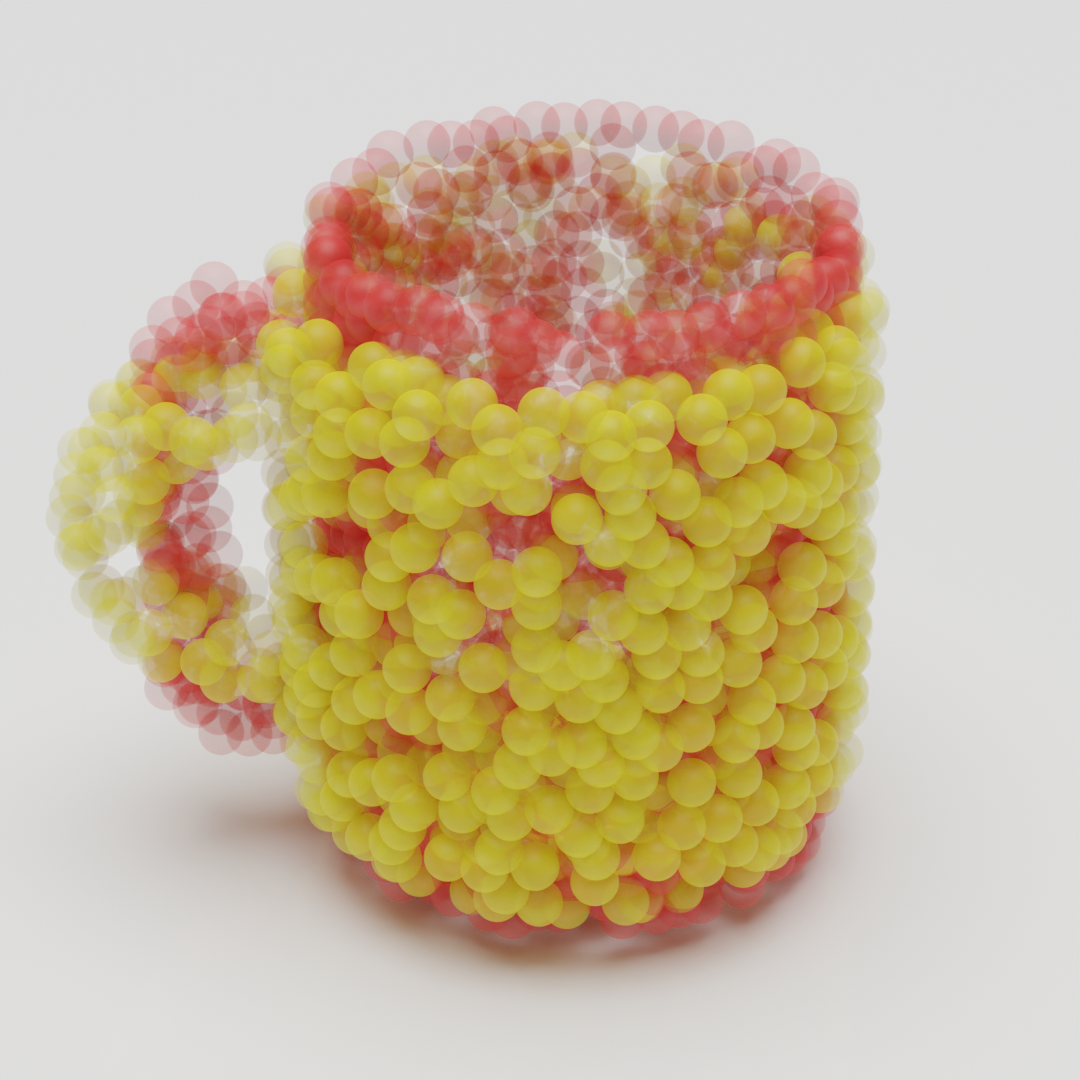
\includegraphics[width=0.24\textwidth]{figures/blender/warp1/canon_over_orig.png}
%     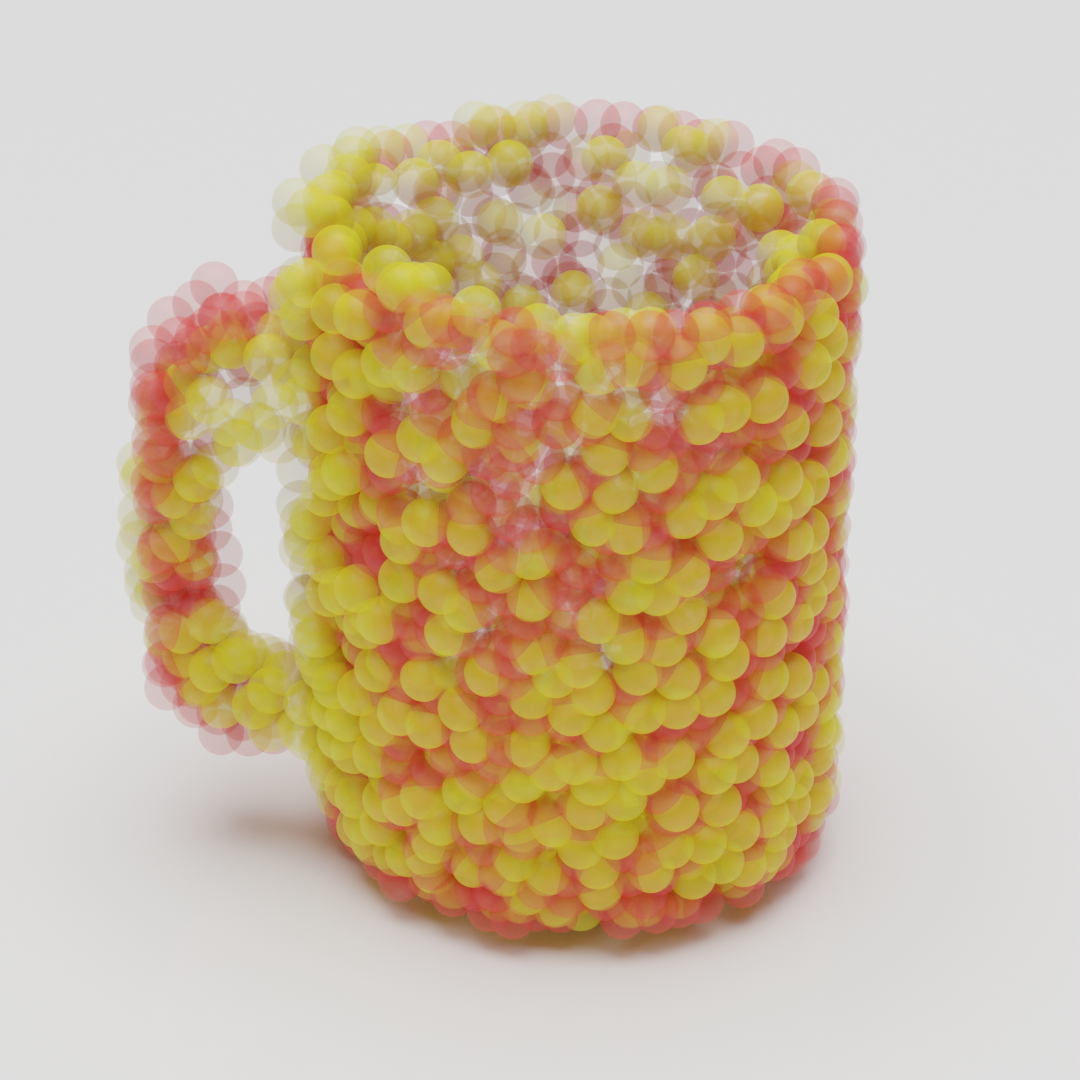
\includegraphics[width=0.24\textwidth]{figures/blender/warp1/warped_over_orig.png}
%     \caption{Source (yellow) and target (red) objects before and after CPD warping.}
%     \label{fig:obj_warp}
%     \vspace{-1em}
% \end{wrapfigure}
Object warping alters the mesh of an object, so that it approximately matches the shape of a different object, usually from the same class. Most object warping approaches turn object meshes into point clouds, which can be warped using techniques from non-rigid Point Set Registration \cite{zhu19Review}. In particular, the Coherent Point Drift (CPD) algorithm \cite{myronenko10point} translates each point in the source point cloud independently, but regularizes the movement of points to be coherent in local regions using frequency-basis regularization. For example, it can warp a small mug onto a larger mug without pulling it inside out, which would be incoherent.

Shape-based Skill Transfer - Warping (SST-W) \cite{thompson21ShapeBased} learns a low-dimensional latent space of object shapes based on the outputs of CPD on a training set. The benefits of SST-W compared to only using object warping are twofold: the latent space can define a generative model of possible object shapes and a gradient decent procedure can be used to fit complete object shapes to partial point clouds. We review their algorithm below:

\begin{enumerate}
    \item Construct a point cloud dataset for $K$ example object instances: $D_S = \{ s^{(1)}, s^{(2)}, ..., s^{(K)} \}$.
    \item Find the canonical point cloud $s^{(C)} \in D_S$, which can be warped to the instances in $D_S \setminus \{s^{(T)}\}$ with the lowest cost using CPD.
    \item Use CPD to warp the canonical $s^{(C)}$ to $s^{(i)}$ and represent the displacement of each point in $s^{(C)}$ as a matrix $W_{T \rightarrow i}$. The shape of $W_{T \rightarrow i}$ is $N{\times}3$, where $N$ is the number of points in $s^{(C)}$. The ordering of points is arbitrary and fixed. Repeat for all instances: $D_W = \{ W_{T \rightarrow 1}, ..., W_{T \rightarrow T - 1}, W_{T \rightarrow T + 1}, ..., W_{T \rightarrow K} \}$.
    \item Flatten the matrices to vectors in $D_W$ and perform Principal Component Analysis. The result is a linear projection $L$ from a high-dimensional space of point displacements to a low-dimensional latent space. $L: \mathbb{R}^{3N} \rightarrow \mathbb{R}^{D_{\mathrm{PCA}}}$.
    \item Given a new, possibly partial, point cloud $s^{(K+1)}$, use gradient descent to minimize a one-sided version of the Chamfer distance \cite{fan17point} between $s^{(K+1)}$ and $s^{(C)} + \theta L^T$ with respect to a latent vector $\theta \in \mathbb{R}^{D_{PCA}}$. $\theta$ represents the shape of the $(K+1)$th object instance and $s^{(C)} + \theta L^T$ is a completed point cloud.
\end{enumerate}

\section{Problem Statement: $\mathrm{SE(3)}$ Object Re-arrangement}

We formulate the object re-arrangement problem as a problem of predicting a pair of 3D homogenous transforms $(T_\mathrm{pick}, T_\mathrm{rel})$ given an initial segmented point cloud of the scene. The transform $T_\mathrm{pick}$ defines the pose of the robot's gripper that results in a successful pick. Moreover, the way the robot is holding the object should be compatible with the task it is to accomplish. E.g. a mug should be held by the rim so that it can be placed on a mug tree by its handle. The transform $T_\mathrm{rel}$ represents the relative transform between the initial pose of the manipulated object and its target pose. For the mug-tree problem, we have, informally, $T_{\mathrm{mug-on-tree}} = T_\mathrm{rel} T_{\mathrm{mug-on-ground}}$. Our problem statement is alike \cite{simeonov22Neurala,simeonov22SE}, whereas \cite{pan22TAXPose} consider only the prediction of $T_\mathrm{rel}$. Our work as well as \cite{simeonov22Neurala,simeonov22SE,pan22TAXPose} solve tasks using open-loop policies; we discuss an extension of our method to closed-loop manipulation in the Conclusion.

\section{Method: SA-Warp}

\begin{algorithm}[H]

\caption{Warp Learning}\label{alg:warp_learn} 

\begin{flushleft}
    \hspace*{\algorithmicindent} \textbf{Input:} Meshes of $K$ example object instances $\{ \mathrm{obj}_1, \mathrm{obj}_2, ..., \mathrm{obj}_K \}$. \\
    \hspace*{\algorithmicindent} \textbf{Output:} Canonical point cloud, vertices and faces and a latent space of warps. \\
    \hspace*{\algorithmicindent} \textbf{Parameters:} Smoothness of CPD warping $\alpha$ and number of PCA components $L$.
\end{flushleft}

\begin{algorithmic}[1]

    \State $\mathrm{PCD} = \left< \mathrm{SampleS}(\mathrm{obj}_i) \right>_{i=1}^K$. \Comment{\textcolor{blue}{Sample a small point cloud per object (Appendix \ref{appendix:method:sampling}).}}
    \State $C = \mathrm{SelectCanonical}(\mathrm{PCD})$. \Comment{\textcolor{blue}{Select a canonical object with index $C$ (Appendix \ref{appendix:method:canonical}).}}
    \State $\mathrm{canon} = \mathrm{Concat}(\mathrm{obj}_C.\mathrm{vertices}, \mathrm{SampleL}(\mathrm{obj}_C))$. \Comment{\textcolor{blue}{Use both vertices and surface samples.}}
    \For {$i \in \{ 1, 2, ..., K \}, i \neq C$}
        \State $W_{C \rightarrow i} = \mathrm{CPD}(\mathrm{canon}, \mathrm{PCD}_i, \alpha)$. \Comment{\textcolor{blue}{Coherent Point Drift warping (Section \ref{sec:background}).}}
    \EndFor
    \State $D_W = \{ \mathrm{Flatten}(W_{C \rightarrow i}) \}_{i = 1, i \neq C}^K$. \Comment{\textcolor{blue}{Dataset of displacements of $\mathrm{canon}$.}}
    \State $\mathrm{PCA} = \mathrm{FitPCA}(D_W, \mathrm{n\_components}=L)$. \Comment{\textcolor{blue}{Learn a latent space of canonical object warps.}}
    \State \Return $\mathrm{Canon}\left(\mathrm{points} = \mathrm{canon}, \mathrm{vertices} = \mathrm{obj}_C.\mathrm{vertices}, \mathrm{faces} = \mathrm{obj}_C.\mathrm{faces}\right), \mathrm{PCA}$.

\end{algorithmic}

\end{algorithm}

\begin{algorithm}[H]

\caption{Warp Inference and Mesh Reconstruction}\label{alg:warp_infer} 

\begin{flushleft}
    \hspace*{\algorithmicindent} \textbf{Input:} Observed point cloud $\mathrm{pcd}$, canonical object $\mathrm{canon}$ and latent space $\mathrm{PCA}$. \\
    \hspace*{\algorithmicindent} \textbf{Output:} Predicted latent shape $v$ and pose $T$. \\
    \hspace*{\algorithmicindent} \textbf{Parameters:} Number of random starts $S$, number of gradient descent steps $T$, learning rate $\eta$ and object size regularization $\beta$.
\end{flushleft}

\begin{algorithmic}[1]

    \State $t_{\mathrm{global}} = \mathrm{Mean}(\mathrm{pcd}, \mathrm{dim}=0)$.
    \State $\mathrm{pcd} = \mathrm{pcd} - t_{\mathrm{global}}$. \Comment{\textcolor{blue}{Center the point cloud.}}
    \For {$i \in \{ 1, 2, ..., S \}$}
        \State $R_{\mathrm{init}} \leftarrow$ Random initial 3D rotation matrix.
        \State Initialize $v = [0]*L, t_{\mathrm{local}} = [0]*3, r = [[1, 0, 0], [0, 1, 0]], s = [1]*3$.
        \State Initialize $\mathrm{Adam}$ \cite{kingma15adam} with parameters $v, t_{\mathrm{local}}, r, s$ and learning rate $\eta$.
        \For {$j \in \{ 1, 2, ..., T \}$}
            \State $\delta = \mathrm{PCA.inverse\_transform}(v)\mathrm{.reshape(-1, 3)}$.
            \State $X = \mathrm{canon.points} + \delta$. \Comment{\textcolor{blue}{Warped canonical point cloud.}}
            \State $R = \mathrm{GramSchmidt(r)}$.
            \State $X = (X * s) R_{\mathrm{init}}^T R^T + t_{\mathrm{local}}$. \Comment{\textcolor{blue}{Scaled, rotated and translated point cloud.}}
            \State $\mathcal{L} = \sum_k^{|\mathrm{pcd}|} \min_l^{|X|} \norm{\mathrm{pcd}_k - X_l}_2^2$. \Comment{\textcolor{blue}{One-sided Chamfer distance.}}
            \State $\mathcal{L} = \mathcal{L} + \beta \max_l^{|X|} \norm{X_l}_2^2$. \Comment{\textcolor{blue}{Object size regularization.}}
            \State Take a gradient step to minimize $\mathcal{L}$ using $\mathrm{Adam}$.
        \EndFor
    \EndFor
    \State Find parameters $v^*, t^*_{\mathrm{local}}, R_{\mathrm{init}}^*, R^*, s^*$ with the lowest final loss across $\{ 1, 2, ..., S \}$.
    \State $X = \mathrm{canon.points} +\mathrm{PCA.inverse\_transform}(v^*)\mathrm{.reshape(-1, 3)}$.
    \State $X = (X * s^*) R_{\mathrm{init}}^{*T} R^{*T} + t^*_{\mathrm{local}} + t_{\mathrm{global}}$. \Comment{\textcolor{blue}{Complete point cloud in workspace coordinates.}}
    \State $\mathrm{vertices} = X[:|\mathrm{canon.vertices}|]$. \Comment{\textcolor{blue}{First $|\mathrm{canon.vertices}|$ points of $X$ are vertices.}}
    \State \Return $\mathrm{Mesh}(\mathrm{vertices} = \mathrm{vertices}, \mathrm{faces} = \mathrm{canon.faces})$. \Comment{\textcolor{blue}{Warped mesh.}}

\end{algorithmic}

\end{algorithm}

In this section, we propose a method, SA-Warp, for behavior cloning of $\mathrm{SE(3)}$ object re-arrangement policies from a single demonstration. Our method has three main components that make it work on a real-world robot: (1) hybrid mesh and point cloud warping to enable the detection of contact points and collision avoidance during motion planning, (2) joints estimation of object shape and pose in 3D using gradient descent and (3) cloning of contact points and nearby points to enable transfer of pick and place actions across object instances.

\begin{figure}
    \centering
    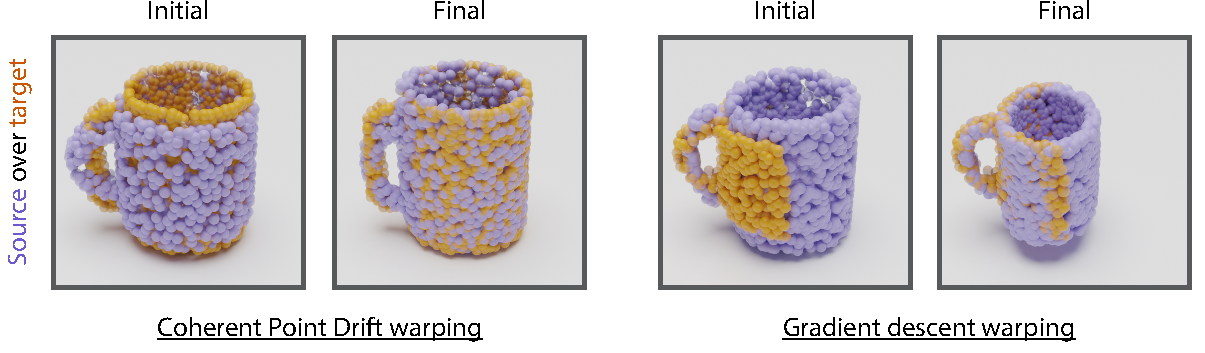
\includegraphics[width=\textwidth]{figures/warping.pdf}
    \caption{Example of warping using CPD and gradient descent with a latent space of warps of a canonical mug. Gradient descent warping works with partial point clouds.}
    \label{fig:latent}
\end{figure}

\begin{figure}
    \centering
    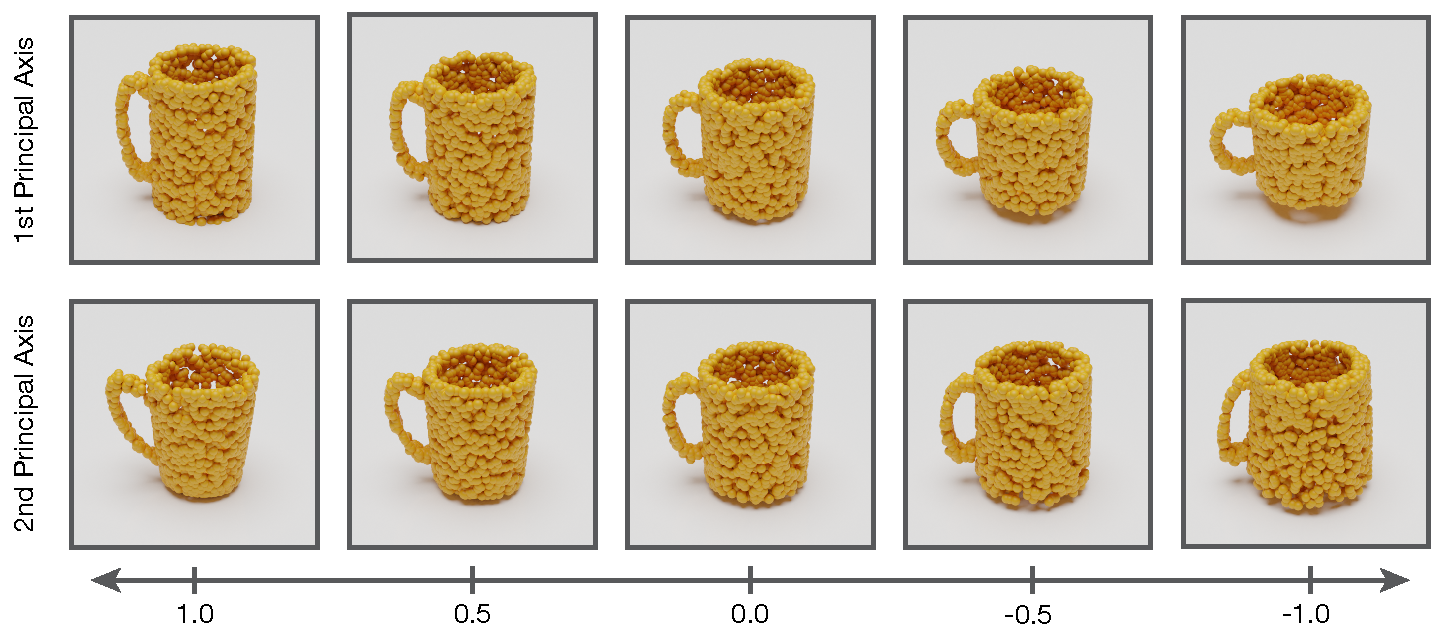
\includegraphics[width=\textwidth]{figures/latent_mugs.pdf}
    \caption{Traversing the latent space of warps of a canonical mug. We show the first two out of eight principal components.}
    \label{fig:latent}
\end{figure}

\begin{figure}
    \centering
    \begin{subfigure}[b]{0.25\textwidth}
        \centering
        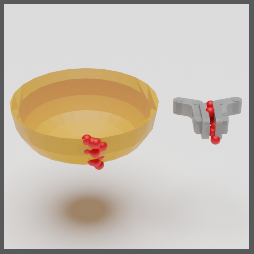
\includegraphics[width=\textwidth]{figures/contact_fig1.pdf}
        \caption{}
    \end{subfigure}
    \hspace{0.05\textwidth}
    \begin{subfigure}[b]{0.25\textwidth}
        \centering
        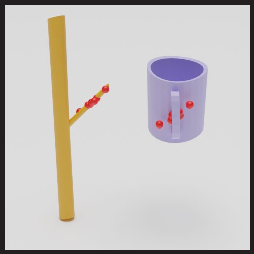
\includegraphics[width=\textwidth]{figures/contact_fig3.pdf}
        \caption{}
    \end{subfigure}
    \hspace{0.05\textwidth}
    \begin{subfigure}[b]{0.25\textwidth}
        \centering
        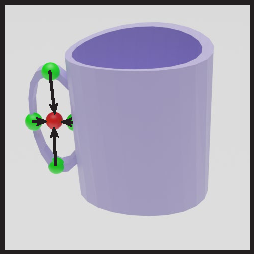
\includegraphics[width=\textwidth]{figures/contact_fig2.pdf}
        \caption{}
    \end{subfigure}
    \caption{(a) Contacts between a gripper and a bowl extracted from a demonstration. (b) Nearby points between a mug and a tree extracted from a demonstration of hanging the mug on the tree. (c) A virtual point (red) representing the branch of the tree intersection the handle of the mug. The red point anchored to the mug using k nearest neighbors on the mug (four are shown in greed) and moves as the mug warps. Note that all points shown in this visualization are extracted automatically.}
    \label{fig:contacts}
\end{figure}

\begin{figure}
    \centering
    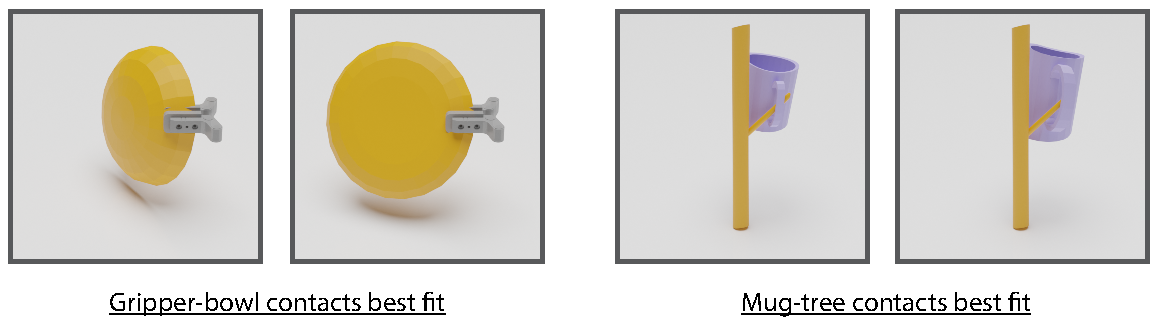
\includegraphics[width=\textwidth]{figures/picks_and_places.pdf}
    \caption{}
    \label{fig:latent}
\end{figure}

\begin{figure}
    \centering
    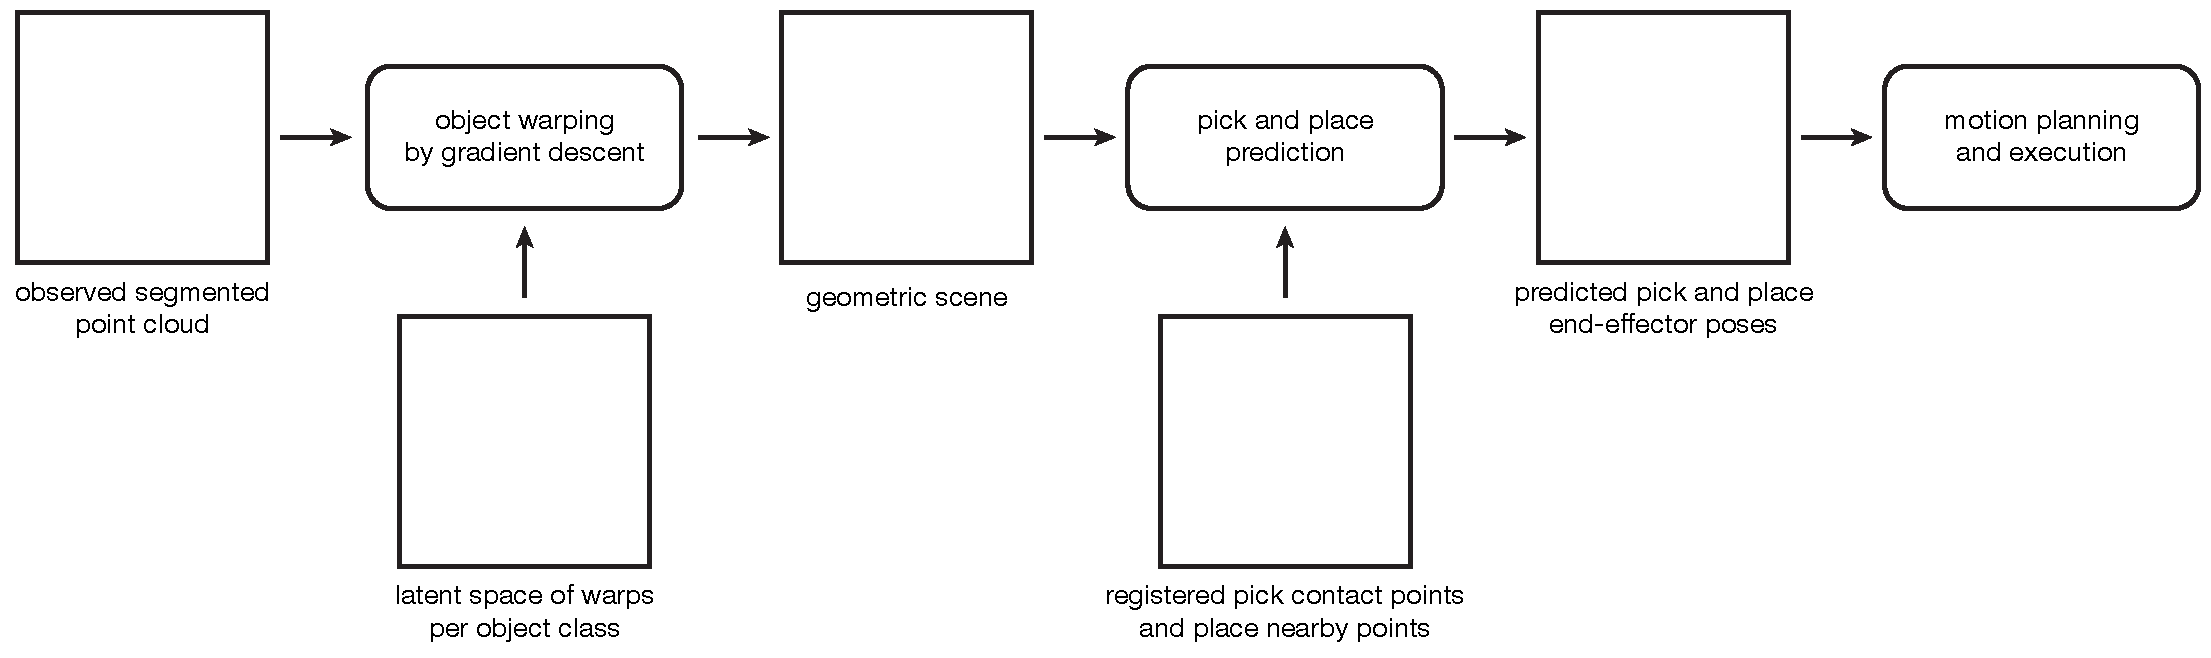
\includegraphics[width=\textwidth]{figures/method_figure.pdf}
    \caption{Main method figure. I'll fill it in with real-world images later.}
    \label{fig:latent}
\end{figure}

\subsection{Hybrid Point Cloud and Mesh Warping}
\label{sec:methods:mesh}



\subsection{Mesh Warping and Pose Estimation in $\mathrm{SE}(3)$}
\label{sec:methods:scene}

\ob{-- Work in progress. -- }

We start with SST-W as a method for learning a latent space of object shape. Our first contribution is in using SST-W as both an object warping and pose estimation method. SST-W assumes that objects appear in a canonical position and orientation (e.g. the handle of the mug always needs to point in the same direction). But, this assumption is unrealistic for general robotic manipulation. We demonstrate that an object template can be translated, rotated and warped at the same time using the gradient descent procedure from Step 5 with multiple random restarts. \evdp{Some context here may be helpful, e.g. why would we expect multiple random restarts to solve the canonical position assumption?} 

\begin{enumerate}
    \item Pick a random initial rotation matrix $R$ from SO(3) (general rotations in space) or SO(2) (planar rotations). Initialize a position offset $C_{\text{local}} \in \mathbb{R}^3$ with zeros.
    \item Compute the center of the new, partial point cloud $s^{(K+1)}$. Call it $C_{\text{global}} \in \mathbb{R}^3$.
    \item Perform gradient descent on the one-sided Chamfer distance between $s^{(K+1)}$ and $(s^{(T)} + \theta L^T) R^T + C_{\text{global}} + C_{\text{local}}$. Optimize the latent object shape $\theta$, the object orientation $R$ and the object offset $C_{\text{local}}$. For brevity, $C = C_{\text{local}} + C_{\text{global}}$.
    \item Repeat the procedure $M$ times and pick the solution with the lowest Chamfer distance.
\end{enumerate}

Intuitively, $\theta$ tells us about e.g. the mug's shape, $R$ tells us where its handle is pointing, $C_{\text{global}}$ tells us where the mug is in the world and $C_{\text{local}}$ accounts for partial observability. To elaborate, we might see exactly half of the mug and therefore $C_{\text{global}}$ is not located in the actual center of the mug, which we account for with $C_{\text{local}}$.
\lsw{This could use a figure to visualize/explain.}

\subsection{Warping of Pick and Place Actions}
\label{sec:methods:cloning}

-- \ob{Work in progress.} --

We assume to have a single demonstration of each task we wish to solve. The demonstration consists of a sequence of recorded pick and place actions \evdp{how many pick and place actions and how many objects do we assume to have in the sequence}. We assume to have a snapshot of the scene right before the robot closes its gripper during pick and right before the robot opens its gripper during placement. Formally, we have a sequence $\left(T_{\text{pick/place}}, (\theta_k, R_k, C_k)_{k=1}^M\right)_{t=1}^T$ of pick/place poses and a representation of all objects in the scene described in Section \ref{sec:methods:scene}. $M$ is the number of objects in the scene and $T$ is the number of time steps in the demonstration.

To clone a \textbf{pick action} between different shapes and poses of the target object, we register a single point on the \textit{canonical object transformed and warped to confirm to the target object}. I.e. for the $k$th object, $PC = (s^{(T)} + \theta_k L^T) R_k^T + C_k$ is its completed point cloud created by canonical object warping. We find the $i$th point in $PC$ that is the closest to the center point between the gripper's two fingers. We also save the orientation of the gripper. When we transfer to a new scene, we have a different instance of an object of the same category in different position and orientation. Denote its completed point cloud $PC'$. We can then execute the pick action at location $PC'_i$ with the grippers orientation rotated by $R'$. Intuitively, the point at which we execute the pick action moves as we warp the canonical object to confirm to different instances of an object. \evdp{Iirc, this is a very important part of the paper. Can we add a Figure 1 that intuitively explains this concept with example objects?}
\lsw{Agreed that a figure is crucial.}
Moreover, we use the orientation of the new object to transform the grasp pose enabling generalization to different object poses.

To clone a \textbf{place action}, we identify pairs of contact points between the in-hand object and whatever we are placing it on. For example, when placing a mug upside down on a counter, we would identify pairs of mug rim and counter points that are touching. When placing a mug on a mug tree, we find points on the branch of the tree that intersect the handle of the mug (by looking at the convex hull of the mug). In this case, there is no contact between the mug and the tree \evdp{why not?}. However, for downstream object warping and pose matching, we would like to always have pairs of mug and tree points that touch. Hence, we add \textit{virtual points} to the point cloud of the mug, which are the intersecting points we found previously expressed in the reference frame of the mug. In order to warp these virtual contact points to different mug instances, we need to \textit{anchor} them to the point cloud of the mug. We do so by finding $k$ nearest neighbors $(n^i_1, ..., n^i_k)$ in the in-hand object for each virtual point $v_i$. We then save the deltas between $v_i$ and its neighbors $\delta_i = (v_i - n^i_1, ..., v_i - n^i_k)$ (Figure \ref{fig:virtual_points}).

The contact points on the placement objects and the virtual points on the in-hand object are registered on the warped canonical objects, analogously to how we register pick points. To transfer to a scene with novel object instances, we can simply warp the canonical objects to conform to the observed point clouds. The only difficulty is with the virtual points, which we do not know how to warp. Hence, we take the nearest neighbors $(n^i_1, ..., n^i_k)$ from the warped canonical point clouds $PC'$ and average their deltas:
\begin{align}
    v'_i = \frac{1}{k} \sum_{j=1}^k n^i_j + \delta_j.
\end{align}

Using the above method, we receive pairs of contact points in a novel scene. We solve for the transformation of the in-hand object so that the contact points are in the best possible alignment \ob{find reference to the algorithm}. Finally, we solve for a collision free motion plan that places the in-hand object to the target pose.

\section{Experiments}

\begin{figure}
    \centering
    \includegraphics[width=0.8\linewidth]{figures/real_testing_mugs.pdf}
    \caption{Caption}
    \label{fig:my_label}
\end{figure}

% \begin{table}[]
%     \centering
%     \begin{tabular}{llll}
%         \toprule
%          Setting & \multicolumn{3}{c}{Success Rate (\%)} \\
%           & Ours & NDF & R-NDF \\
%          \midrule
%          Mug-tree $\mathrm{SE}(2)$ fixed tree & 100\% & - & - \\ 
%          Mug-tree $\mathrm{SE}(3)$ fixed tree & - & - & - \\ 
%          Mug-tree $\mathrm{SE}(2)$ & 100\% & - & - \\ 
%          Mug-tree $\mathrm{SE}(3)$ & - & - & - \\ 
%          \bottomrule
%     \end{tabular}
%     \caption{Caption \ob{Turn into a barchart.}}
%     \label{tab:my_label}
% \end{table}

\begin{table*}[t!]
    \centering
    \begin{tabular}{lcccccc}
        \toprule
          & \multicolumn{2}{c}{\textbf{Mug on Tree}} & \multicolumn{2}{c}{\textbf{Bowl on Mug}} & \multicolumn{2}{c}{\textbf{Bottle in Container}} \\
         \textbf{Method} & Upright & Arbitrary & Upright & Arbitrary & Upright & Arbitrary \\
         \midrule
         NDF$^1$ & 64\%** & - & - & - & - & - \\
         R-NDF$^2$ & - & - & - & - & - & - \\
         \textbf{SA-Warp} & 100\%* & 100\%* & - & - & - & - \\
         \bottomrule
    \end{tabular}
    \caption{Success rates of \hl{real-world} pick-and-place experiments. $^1$The target object (e.g. the mug tree) is in a fixed pose for this experiment. $^2$As measured for the open-source version of \citet{simeonov22Neurala}. * Small number of trials. ** Old setup.}
    \label{tab:real_world}
\end{table*}

\begin{table}[h]
    \centering
    \begin{tabular}{lcccccc}
        \toprule
          & \multicolumn{2}{c}{\textbf{Mug on Tree}} & \multicolumn{2}{c}{\textbf{Bowl on Mug}} & \multicolumn{2}{c}{\textbf{Bottle in Container}} \\
         \textbf{Method} & Upright & Arbitrary & Upright & Arbitrary & Upright & Arbitrary \\
         \midrule
         R-NDF$^1$ & 84.0 & 75.0 & 74.0 & 70.0 & 80.0 & \textbf{75.0} \\
         R-NDF$^2$ & 71.0 & 70.0 & 69.0 & 60.0 & 81.0 & 59.0 \\
         \textbf{SA-Warp} & \textbf{85.0} & \textbf{82.0} & \textbf{81.0} & \textbf{78.0} & \textbf{88.0} & 69.0 \\
         \bottomrule
    \end{tabular}
    \caption{Success rates of predicted target poses of objects in \hl{simulation}. Upright and arbitrary starting object poses. $^1$As reported in \citet{simeonov22Neurala}. $^2$As measured for the open-source version of \citet{simeonov22Neurala}.}
\end{table}
\begin{table}[h]
    \centering
    \begin{tabular}{lccc}
        \toprule
         \textbf{Method} & \# Train. Objects & \# Demos. & Labels \\
         \midrule
         NDF & 200 & 5-10 & Yes \\
         R-NDF & 200 & 5-10 & Yes \\
         TAX-Pose & 200 & 5-10 & No \\
         \textbf{SA-Warp} & \textbf{10} & \textbf{1} & \textbf{No} \\
         \bottomrule
    \end{tabular}
    \caption{Required training objects, training demonstrations and additional labeled data across methods.}
    \label{tab:training}
\end{table}

% \begin{figure*}[]
%     \centering
%     \begin{subfigure}{(\linewidth - 0.1\linewidth)/6}
%         \centering
%         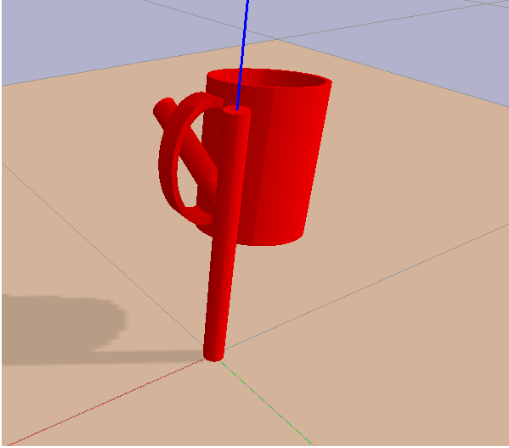
\includegraphics[width=\linewidth]{figures/virtual/1.png}
%         \caption{}
%     \end{subfigure}
%     \begin{subfigure}{(\linewidth - 0.1\linewidth)/6}
%         \centering
%         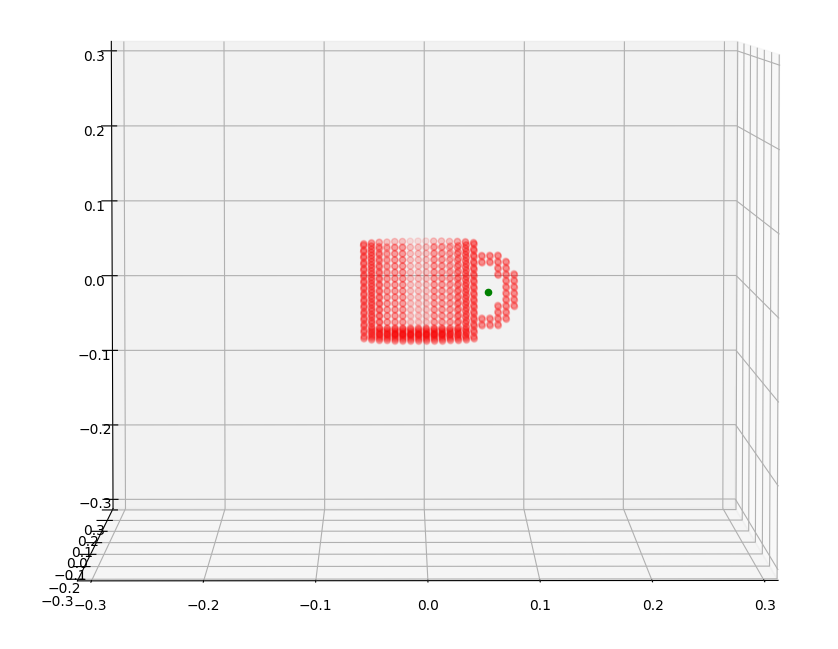
\includegraphics[width=\linewidth]{figures/virtual/2.png}
%         \caption{}
%     \end{subfigure}
%     \begin{subfigure}{(\linewidth - 0.1\linewidth)/6}
%         \centering
%         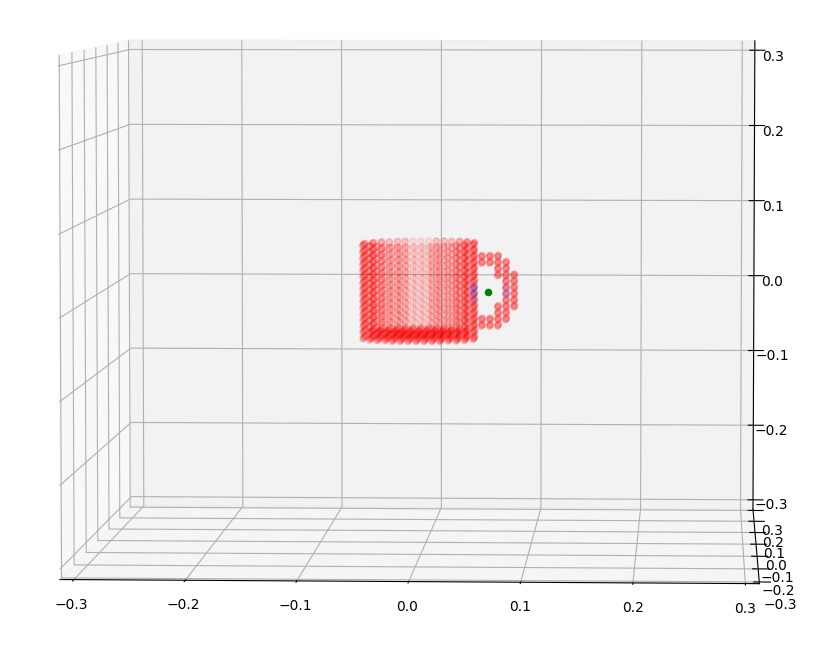
\includegraphics[width=\linewidth]{figures/virtual/3.png}
%         \caption{}
%     \end{subfigure}
%     \begin{subfigure}{(\linewidth - 0.1\linewidth)/6}
%         \centering
%         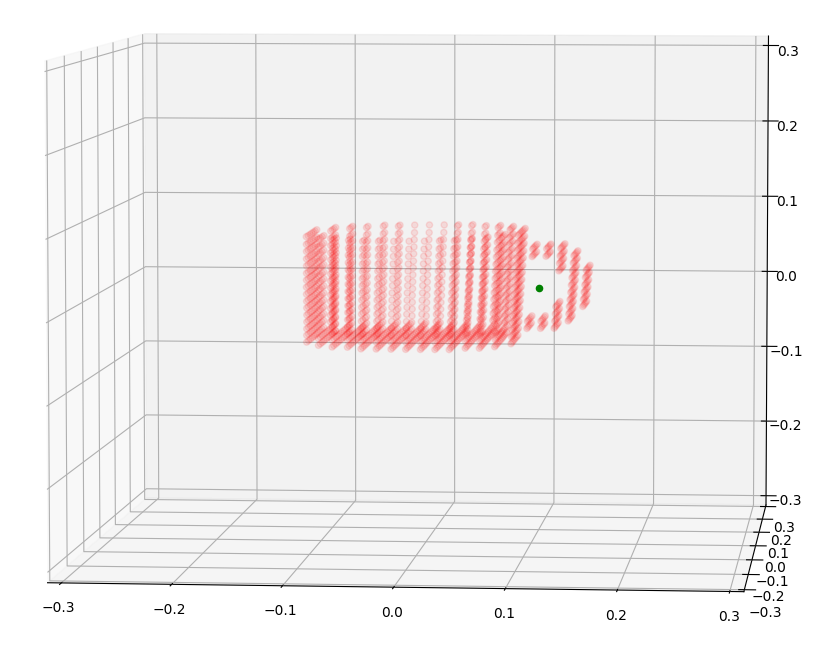
\includegraphics[width=\linewidth]{figures/virtual/4.png}
%         \caption{}
%     \end{subfigure}
%     \begin{subfigure}{(\linewidth - 0.1\linewidth)/6}
%         \centering
%         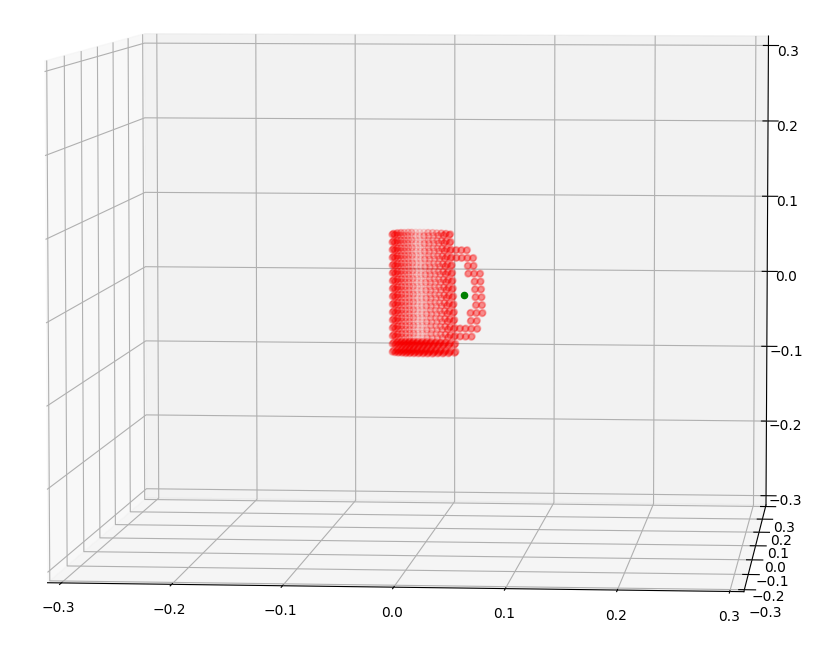
\includegraphics[width=\linewidth]{figures/virtual/5.png}
%         \caption{}
%     \end{subfigure}
%     \begin{subfigure}{(\linewidth - 0.1\linewidth)/6}
%         \centering
%         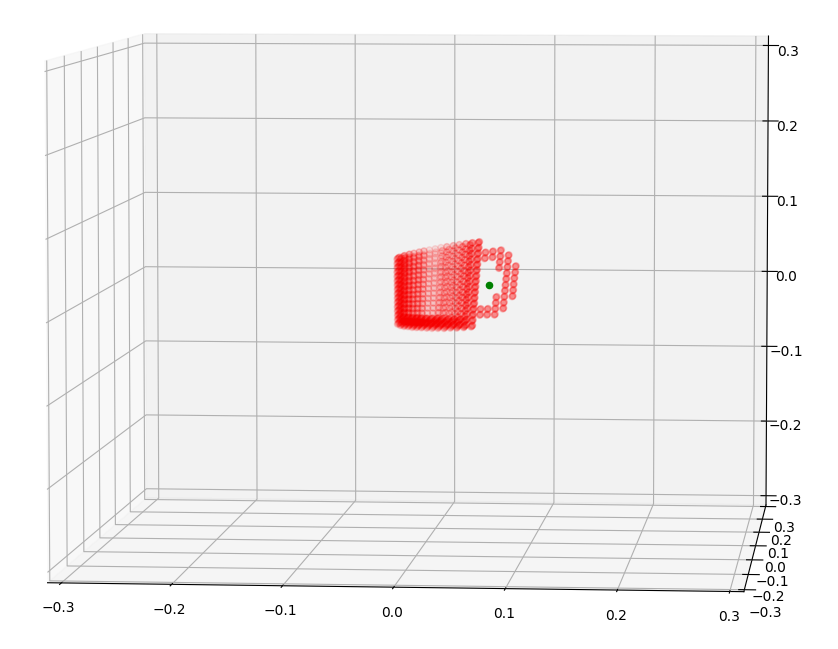
\includegraphics[width=\linewidth]{figures/virtual/6.png}
%         \caption{}
%     \end{subfigure}
%     \caption{Sketch: (a): a demonstration of the mug tree task, (b) a virtual point (green) in the middle of the mug's handle, (c) 10 (?) nearest neighbors (blue\ob{almost invisible, I know}), (d-f) warping the virtual point together with the mug.}
%     \label{fig:virtual_points}
% \end{figure*}

\section{Limitations}

Uniformity: SST-W requires the distribution of points on the canonical object and the observed object to be approximately uniform. This can be achieved by subsampling the (usually quite large) point cloud using farthest point sampling.

\section{Conclusion}

Object decomposition / part segmentation \cite{tenorth13Decomposing,vahrenkamp16Partbased,chen22Neural}

%===============================================================================

\clearpage

%===============================================================================

% no \bibliographystyle is required, since the corl style is automatically used.
\bibliography{main,zotero}  % .bib

\clearpage
\appendix

\section{Method Details}
\label{appendix:method}

\subsection{Point Cloud Sampling}
\label{appendix:method:sampling}



\subsection{Canonical Object Selection}
\label{appendix:method:canonical}

Among the $K$ example objects, we would like to find the one that is the easiest to warp to the other objects. For example, if we have ten examples of mugs, but only one mug has a square handle, we should not choose it as it might be difficult to warp it to conform to the round handles of the other nine mugs.

\begin{algorithm}[H]

\caption{Exhaustive Canonical Object Selection}\label{alg:canon_select_1} 

\begin{flushleft}
    \hspace*{\algorithmicindent} \textbf{Input:} Meshes of $K$ example object instances $\{ \mathrm{obj}_1, \mathrm{obj}_2, ..., \mathrm{obj}_K \}$. \\
    \hspace*{\algorithmicindent} \textbf{Output:} Canonical object $\mathrm{obj}^C$, $\mathrm{PCA}$ mapping latent vectors to warps of $\mathrm{obj}^C$. \\
\end{flushleft}

\begin{algorithmic}[1]

    \State Construct a point cloud dataset for $K$ example object instances: $D_S = \{ s^{(1)}, s^{(2)}, ..., s^{(K)} \}$
    \State Heuristic $h \leftarrow 0$.
    \State Match objects between $\hat{z}$ and $z^g$ (Section \ref{sec:methods:search}).
    \For {$k$th object}
        \State $d \leftarrow \norm{\hat{z}_k - z^g_k}^2_2$
        \If {$d < \delta$}
            \State $h \leftarrow h + d$. \Comment{Close enough to goal.}
        \ElsIf{$j_{\psi}(\hat{z}_k) = 1$}
            \State $h \leftarrow h + 1$. \Comment{At least one step away from goal.}
        \Else
            \State $h \leftarrow h + 2$. \Comment{At least two steps away from goal.}
        \EndIf
    \EndFor
    \State \Return $h$.

\end{algorithmic}

\end{algorithm}

\begin{algorithm}[H]

\caption{Approximate Canonical Object Selection}\label{alg:canon_select_2} 

\begin{flushleft}
    \hspace*{\algorithmicindent} \textbf{Input:} Meshes of $K$ example object instances $\{ \mathrm{obj}_1, \mathrm{obj}_2, ..., \mathrm{obj}_K \}$. \\
    \hspace*{\algorithmicindent} \textbf{Output:} Canonical object $\mathrm{obj}^C$, $\mathrm{PCA}$ mapping latent vectors to warps of $\mathrm{obj}^C$. \\
\end{flushleft}

\begin{algorithmic}[1]

    \State Predict next state $\hat{z} = z + g_{\theta}(z, a)$.
    \State Heuristic $h \leftarrow 0$.
    \State Match objects between $\hat{z}$ and $z^g$ (Section \ref{sec:methods:search}).
    \For {$k$th object}
        \State $d \leftarrow \norm{\hat{z}_k - z^g_k}^2_2$
        \If {$d < \delta$}
            \State $h \leftarrow h + d$. \Comment{Close enough to goal.}
        \ElsIf{$j_{\psi}(\hat{z}_k) = 1$}
            \State $h \leftarrow h + 1$. \Comment{At least one step away from goal.}
        \Else
            \State $h \leftarrow h + 2$. \Comment{At least two steps away from goal.}
        \EndIf
    \EndFor
    \State \Return $h$.

\end{algorithmic}

\end{algorithm}

\end{document}
